% !TEX root = ../../semexp-thesis.tex

\section{Semantic Object Interfaces for Exploratory Programming}
\label{sec:design/agent}

\begin{figure}
	\centering
	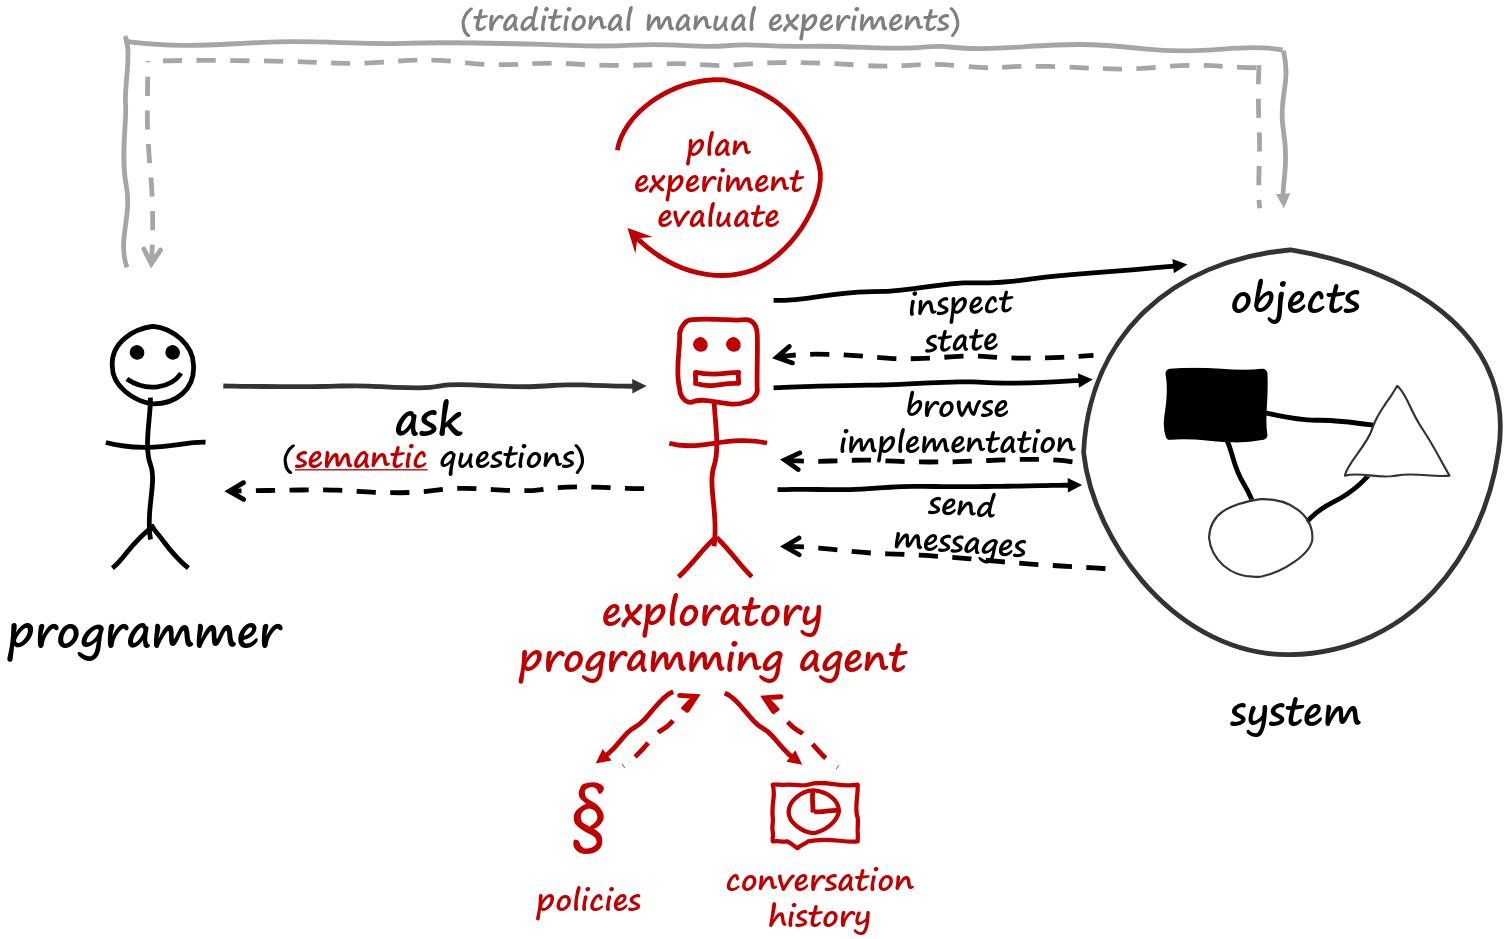
\includegraphics[width=.9\textwidth]{03_agent/framework.png}
	% todo: update figure: use revised vocabulary and darker red. update red reference in this and other captions.
	\caption[Our approach of \emph{semantic object interfaces} for semantic exploratory programming systems.]{
		Our approach of semantic object interfaces for semantic exploratory programming systems.
		The programmer expresses high-level, contextual, and often natural-language questions about an object to the interface and receives answers on the same abstraction level.
		Internally, an \emph{exploratory programming agent} (\bold{\textcolor{red}{red}}) translates these questions and interacts with the system to perform low-level experiments.
	}
	\label{fig:design/agent/framework}
\end{figure}

To delegate parts of the research process to the exploratory programming system, we construct an \emph{exploratory programming agent}, which uses a generative LLM for planning, generating experiments, and communicating with the programmer in natural language.
To connect the agent with the programming system, we propose the design of an \emph{semantic object interface}, which describes the communication between the programmer, the agent, and the system~\cite{thiede2024talking}~(\cref{fig:design/agent/framework}).
Our approach follows the object-oriented paradigm of many programming systems in that semantic object interfaces focus on a single object from the running system.
Thus, semantic object interfaces resemble traditional message sending to objects, and programmers can interact with objects via the agent by the means of natural-language and semantic questions.

As part of this framework, the agent takes high-level and context-dependent \emph{semantic} questions from the programmer and translates them into low-level technical experiments to answer the questions.
Our framework comprises three fundamental actors:

\begin{description}[noextralabelsep]
	\item[The programmer] conducts a larger exploratory research process, from which different questions arise.
	The programmer asks such questions about an object in a system and expects answers on a similar level of abstraction.
	These questions are \emph{semantic} and conceptual, which means they are expressed in the programmer's mental model and vocabulary, typically have an informal or natural-language style, and often depend on the context of previous questions and answers.

	\item[The object] is any object in the system, for example a particular domain object, a code object (such as a class or method), or an artifact from the programming system (such as a call graph, a benchmark, or a program trace).
	It is part of an \emph{object graph}, which embeds it into a larger context of the system.
	It is also linked to an \emph{implementation}, which describes the object's behavior through further objects and may be specified using code, tests, or other forms such as contracts.

	Objects can be accessed either by sending them \emph{messages} (which in many languages is also referred to as \emph{invoking methods}) or through \emph{reflection interfaces} that expose their internal state, implementation, or location in the object graph.

	\item[The exploratory programming agent] is an intelligent mediator between the programmer and the object in the system.
	It automatically translates conceptual questions from the programmer into interactions with the system and translates the results of these interactions back into answers for the programmer.

	Internally, the agent conducts research processes autonomusly: it interprets the programmer's question, develops a plan, designs and conducts experiments, evaluates their results, and repeats as necessary (until all required information has been collected) before delivering a reasoned answer to the questions and returns it to the programmer.

	The agent uses two resources: a set of \emph{policies} and a \emph{conversation history}.
	\emph{Policies} define abstract agent behavior, such as the types and frequency of experiments and the format of answers.
	The \emph{conversation history} consists of past communications with the programmer and experiments from the current conversation.
	It serves as a context for handling subsequent requests.
	Thus, the programmer does not need to repeatedly explicate their intentions in every question but grows a shared vocabulary and knowledge with the agent as the conversation evolves.
\end{description}

\subsection*{Answering Questions through Automated Experiments}

Our framework allows programmers to ask arbitrary questions about objects in a system that can reference two different aspects:

\begin{description}[noextralabelsep]
	\item[Functional questions] (or ``what'' questions) refer to the state of objects and the actual things in the domain they represent.
	They typically constitute inquiries that are or could be covered by regular (analytical) system features or objects' behavior.

	For example, in a sales system, typical functional questions could be ``How many customers are there?'', ``Which product in this category has generated the highest profit in the last quarter?'', or ``What is the age distribution of weekend customers?''.

	\item[Epistemic questions] (or ``how'' questions) refer to the behavior of objects, domain concepts, and their implementation.
	Programmers ask these questions to explore the capabilities of a system, understand the technical foundations, or ideate and prototype new applications.

	For example, in a sales system, epistemic questions could include ``What information do we store about customers?'', ``How is the tagging system for products modeled?'', or ``How can we analyze the shopping behavior of customers?''.

	Note that given the uniform object model of many programming systems, epistemic questions about a domain object equal functional questions about a code object from the implementation of the domain; however, the former perspective provides additional context about the system through a concrete example.
\end{description}

To answer both functional and epistemic questions, the agent automatically conducts experiments by utilizing three types of interfaces that most existing programming systems already offer:

% todo: from feedback: align lengths of items here?
\begin{description}[noextralabelsep]
	\item[State inspection] allows the internal information of objects to be explored, for instance, by looking up a variable or enumerating all properties.
	\item[Implementation browsing] explores the specified behavior of objects\linebreak{}through their \emph{protocols}, \emph{implementation}, and \emph{documentation}.
	\emph{Protocols} refer to the set of messages an object understands.
	\emph{Implementation} includes the source code of objects or classes, but also their integration within the global system through call graphs or related concepts (e.g., senders or program traces) for understanding the usage of objects by example.
	\emph{Documentation} can be provided through comments, examples, or alternative system descriptions.

	Following the singularity of objects and meta objects noted above, implementation browsing of domain objects equals state inspection of their classes, but is associated with a different connotation by adhering to the context of the original object.
	For example, using symbolic execution methods, both the state and effective behavior of objects can explored at once.
	\item[Message sending] constitutes regular communication with objects to activate their behavior.
	As opposed to state inspection and implementation browsing, normal messages can be sent without requiring reflective capabilities.\footnote{From our classification, we exclude special reflective messages such as \code{instVarNamed:} in Smalltalk as well as restricted visibility of messages such as the \code{private} access modifiers in Java.}
\end{description}

Note that the agent generally does not require any manual preparation for specific systems and packages from domain experts or programmers but will learn about the system on its own.
Thus, even to answer simple functional questions, the agent will internally ask and answer epistemic questions to understand the system and domain concepts and preserve the collected knowledge in its internal conversation history.
Analogously, every message send to a previously unknown system is preceded by browsing its implementation, through which the agent discovers the relevant protocols and messages to use.

\begin{example}
	A programmer asks ``Which product has generated the highest profit?'' about a selected shop object.
	In response, the agent first executes a series of experiments by browsing the shop's implementation to explore several messages, classes, and their documentation related to the concepts ``product'' and ``profit'' to understand what these concepts mean and how they are represented in the system.

	After identifying relevant messages such as \code{Shop>>orders}, \code{Order>>\allowbreak productItems}, and \code{Product>>price}, it plans how to combine this information to compute the most profitable product and runs a script that queries the system for this information as another experiment.

	Finally, the agent evaluates the results of this experiment and returns a summarized answer in natural language to the programmer.
	The question was answered and the programmer can continue by asking another question to the agent or performing another exploratory activity.
\end{example}

\subsection*{Integrating Semantic Object Interfaces into Exploratory Programming Systems}
\label{sec:design/agent/interfaces}

To support immediate access to semantic object interfaces from within exploratory programming systems, we aim for tight integration with traditional tools.
For this, we identify two primary interfaces in such systems through which programmers explore objects: \emph{object inspection tools} and \emph{message sending through scripts}.
We propose to extend these interfaces with semantic capabilities: object inspection tools with a \emph{conversation mode} and message sending with a language extension for \emph{semantic messaging}.

\paragraph{A conversation mode for object inspection tools}
\label{par:design/agent/interfaces/inspector}

\begin{figure}
	\centering
	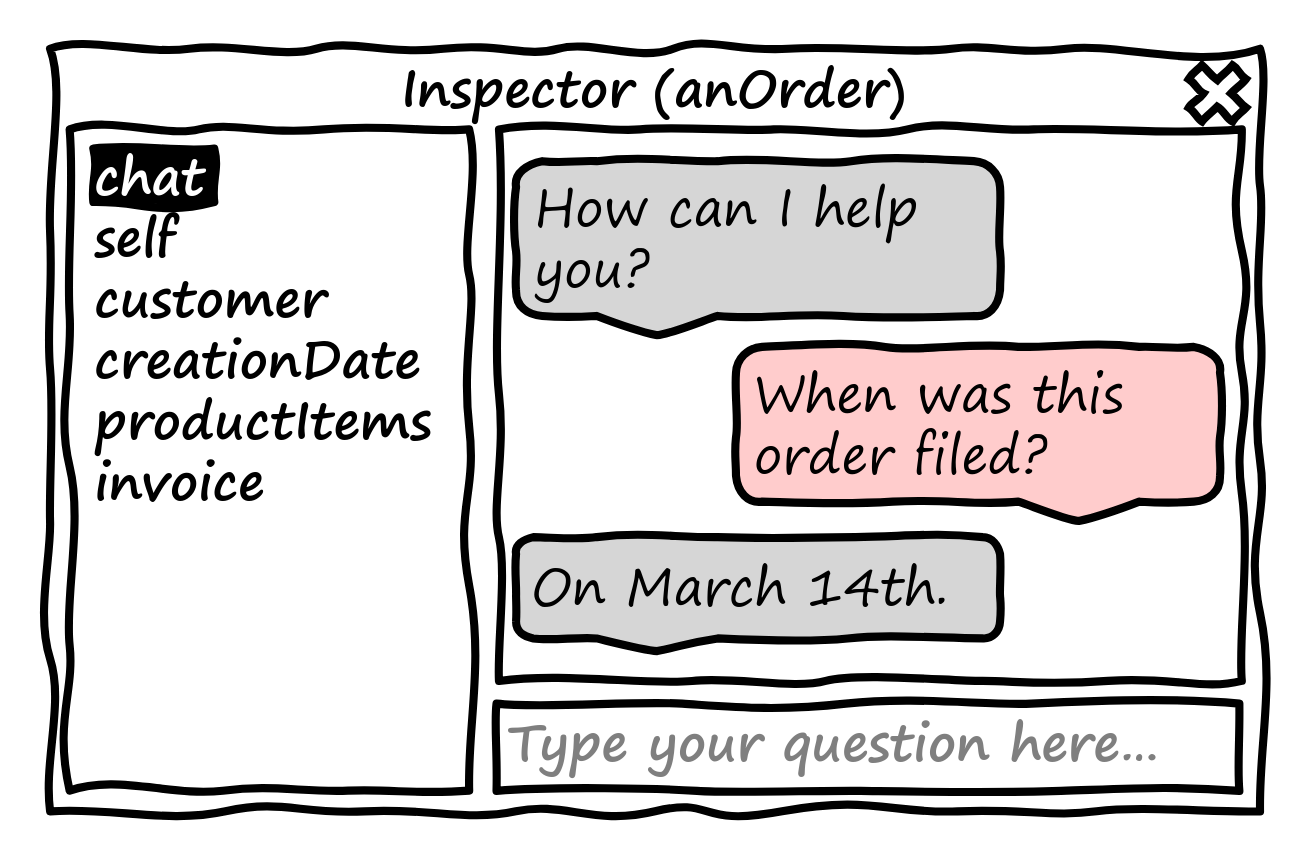
\includegraphics[height=10\baselineskip]{03_agent/inspector.png}
	\caption[Possible integration of a conversational semantic interface into a traditional object inspection tool.]{
		Possible integration of a conversational semantic interface into a traditional object inspection tool.
		Programmers can ask conceptual questions about objects in natural languages besides inspecting their internal state.
	}
	\label{fig:design/agent/interfaces/inspector}
\end{figure}

Inspection tools allow programmers to explore and manipulate the internal state of objects through a list of variables or properties.
We propose a new \emph{conversation mode} in inspection tools that allow programmers to ask semantic questions about an object~(\cref{fig:design/agent/interfaces/inspector}).
Thus, in addition to the usually technical state inspection, they can then also chat with an object through the exploratory programming agent.

Through the chat interface, programmers can express questions in natural language without needing to know the vocabulary and protocols of the object's domain.
Additionally, they can ask follow-up questions in the context of a conversation without repeating or editing their original thoughts, like in a real-life conversation between two programmers.

\paragraph{Semantic messaging in scripts}
\label{par:design/agent/interfaces/messaging}

Scripting is another popular starting point for exploration.
Especially programmers who are proficient in the programming language and familiar with the protocols of a system often prefer message sending through scripts to manually exploring object graphs through inspection tools.
For example, the following Smalltalk script retrieves the product with the highest quantity from a list of order items:

\begin{multicode}
	(self orderItems detectMax: \#quantity) product.
\end{multicode}

We propose an extension to object-oriented scripting languages that allows for \emph{semantic messaging}: similar to pseudocode, programmers can write semantic messages with fictitious names (that do not even have to match the vocabulary of an object) to express their intents but send these messages to objects just like regular messages.
Unlike regular messages, semantic messages do not require an implementation at the receiver object but get processed by an exploratory programming agent, which interprets the message as a question and internally inspects the object or sends it regular messages to determine a return value.
For instance, the above example could be expressed as any of the following:
\begin{multicode}
	self mostOftenBoughtArticle.

	self orderItems theOneWithHighestAmount.
\end{multicode}
Like regular messages, semantic messages can also pass arguments, e.g.:
\begin{multicode}
	aProduct numberOfSalesTo: aCustomer.

	aProduct numberOfSalesFrom: \textquotesingle Q3 2023\textquotesingle{} to: \textquotesingle Q4 2023\textquotesingle.
\end{multicode}

\noindent
Thus, programmers can maintain their scripting flow when asking questions even if they are unaware of certain protocols, and they do not have to express questions using specific protocols and syntax or implement algorithms for more problems.

\ParSep

Semantic object interfaces allow programmers to delegate parts of their research process to the programming system by expressing conceptual questions, letting an exploratory programming agent research them autonomously and map them to low-level experiments, and receiving conceptual answers in natural language.
